\clearpage
\pagenumbering{arabic}
\setcounter{page}{1}

\addtotoc{Товчлол}
\thispagestyle{plain}

\begin{center}
{\large\bfseries \titlename}
\end{center}

\begin{flushright}
\small \departmentname\\
Оюутан: \studentID, \authorShort\\
Удирдагч багш: \supervisorname
\end{flushright}

\setlength{\columnsep}{5mm}
\setlength{\parindent}{0pt}

\begin{multicols}{2}

\small

\textbf{1. Удиртгал}

Орчин үед хүмүүс өдөр тутмын ажил, хичээл,
хувийн төлөвлөгөөгөө тогтмол тэмдэглэх
хэрэгцээ өндөр болсон. Гэвч цаасан
тэмдэглэл алдагдах эрсдэлтэй, авч явахад
хүндрэлтэй, мэдээлэл хайхад төвөгтэй бөгөөд
олон тэмдэглэлийн аппликейшнд сануулга
болон нэмэлт боломж хязгаарлагдмал байдаг.
Иймээс стикер үүсгэдэг, сануулга өгдөг,
календарын харагдац бүхий ухаалаг дижитал
тэмдэглэлийн шийдэл шаардлагатай болсон.
Энэ шаардлагад тулгуурлан энэхүү ажлаар
``AI Notebook'' системийг боловсруулж
хэрэгжүүлэв.

\textbf{Зорилго}

Энэхүү судалгааны ажлын гол зорилго нь
frontend болон backend-д тулгуурласан,
хэрэглэгчийн баталгаажуулалт, тэмдэглэлийн
менежмент, хиймэл оюун ухаанаар стикер
үүсгэх боломж бүхий ухаалаг тэмдэглэлийн
гар утасны аппликейшн зохион бүтээж,
хөгжүүлэн, түүний ажиллагааг туршилтаар
үнэлэхэд оршино.

\textbf{2. Судалгааны арга зүй}

Энэхүү судалгаанд дизайн шинжлэх ухааны
судалгааны арга зүй (Design Science Research)
ашиглаж, шаардлага тодорхойлох, архитектур
төлөвлөх, хөгжүүлэлт хийх, турших,
баталгаажуулах давталтат үе шатыг
хэрэгжүүлсэн.

Арга зүйн түвшинд:
\begin{itemize}
\item Өгөгдлийн урсгалын диаграмм (DFD)
контекст, нэгдүгээр, хоёрдугаар түвшинд
задлан тайлбарласан.
\item Дарааллын диаграмм (Sequence Diagram)
нэвтрэх, тэмдэглэл үүсгэх, стикер үүсгэх,
мэдэгдэл хүргэх урсгалуудыг ажиллуулсан.
\item Интеграцийн тест --- API урсгал, токен
баталгаажуулалт, алдааны урсгал,
гүйцэтгэлийн хэмжилт зэргийг хийсэн.
\end{itemize}

Судалгаанд функционал болон функционал
бус шаардлагуудыг тусад нь тодорхойлж, аль
шаардлага аль модульд хэрэгжсэн, хэрхэн
баталгаажсан зэргийг мөрдөх матрицаар
харуулав.

\vspace{0.2cm}
\begin{flushright}
\textit{\small Хүснэгт 2.1 Функционал шаардлагын мөрдөх матриц}
\end{flushright}
\vspace{-0.2cm}
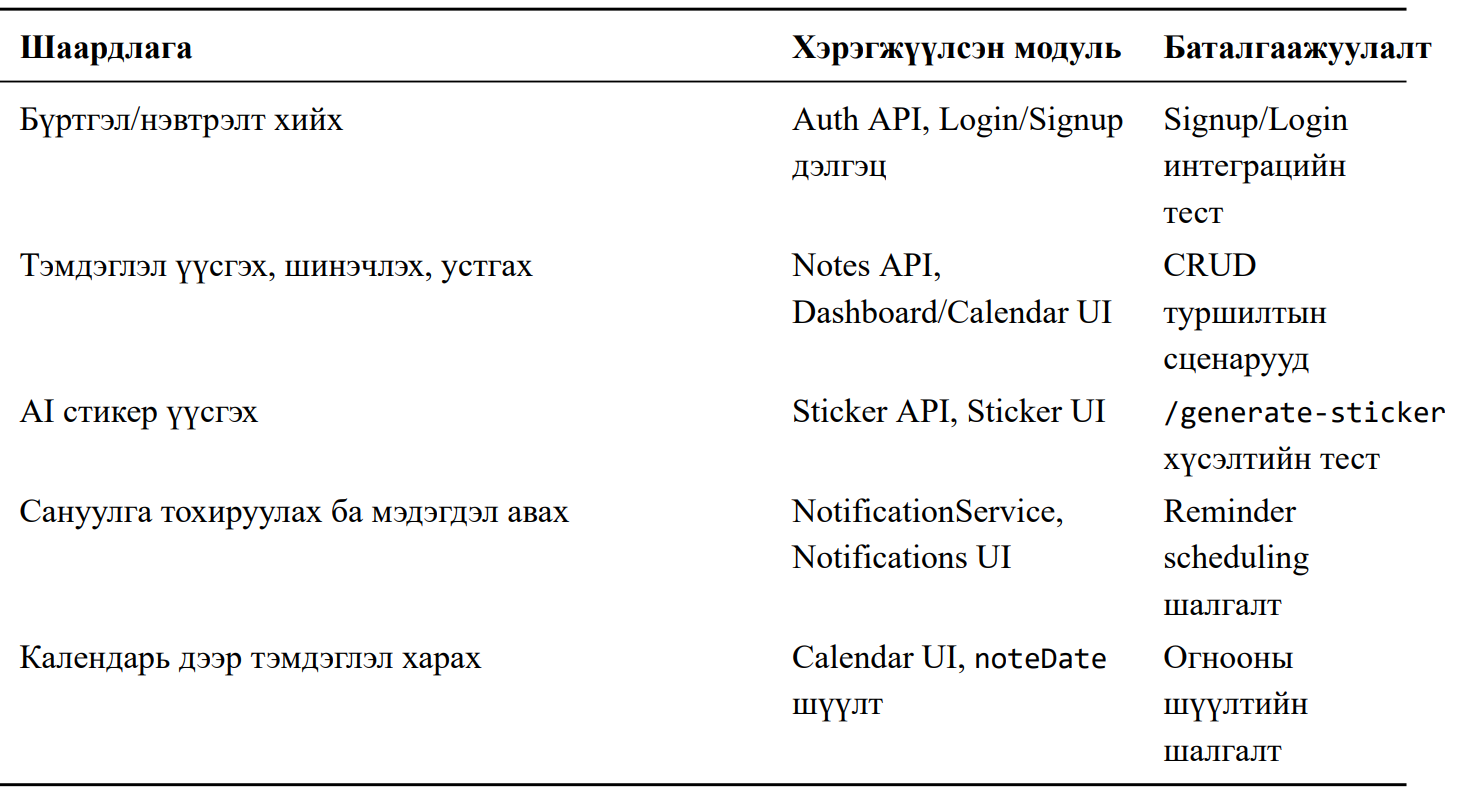
\includegraphics[width=\columnwidth]{Pictures/11.png}

Мөн өгөгдлийн урсгалыг контекст түвшнээс
эхлэн шаталсан (DFD level 0--2) байдлаар
задлан тайлбарлаж, хэрэглэгчийн үйлдлээс
эхлээд өгөгдлийн сан болон хиймэл оюуны
үйлчилгээ хүртэлх урсгалыг тодорхойлсон.
Доор контекст түвшин болон нэгдүгээр
түвшинийг харуулав.

\vspace{0.2cm}
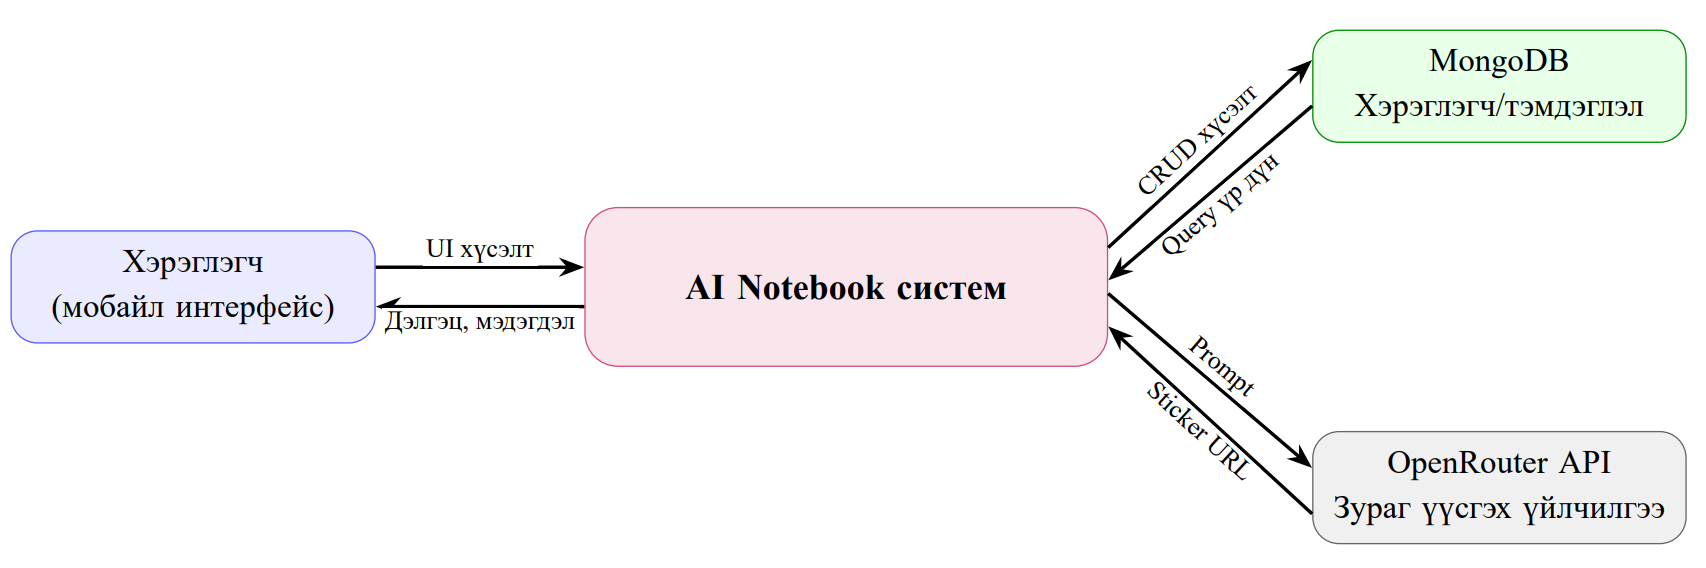
\includegraphics[width=\columnwidth]{Pictures/12.png}
\begin{flushright}
\textit{\small Зураг 2.1 Контекст түвшний өгөгдлийн урсгалын зураг}
\end{flushright}

\vspace{0.2cm}
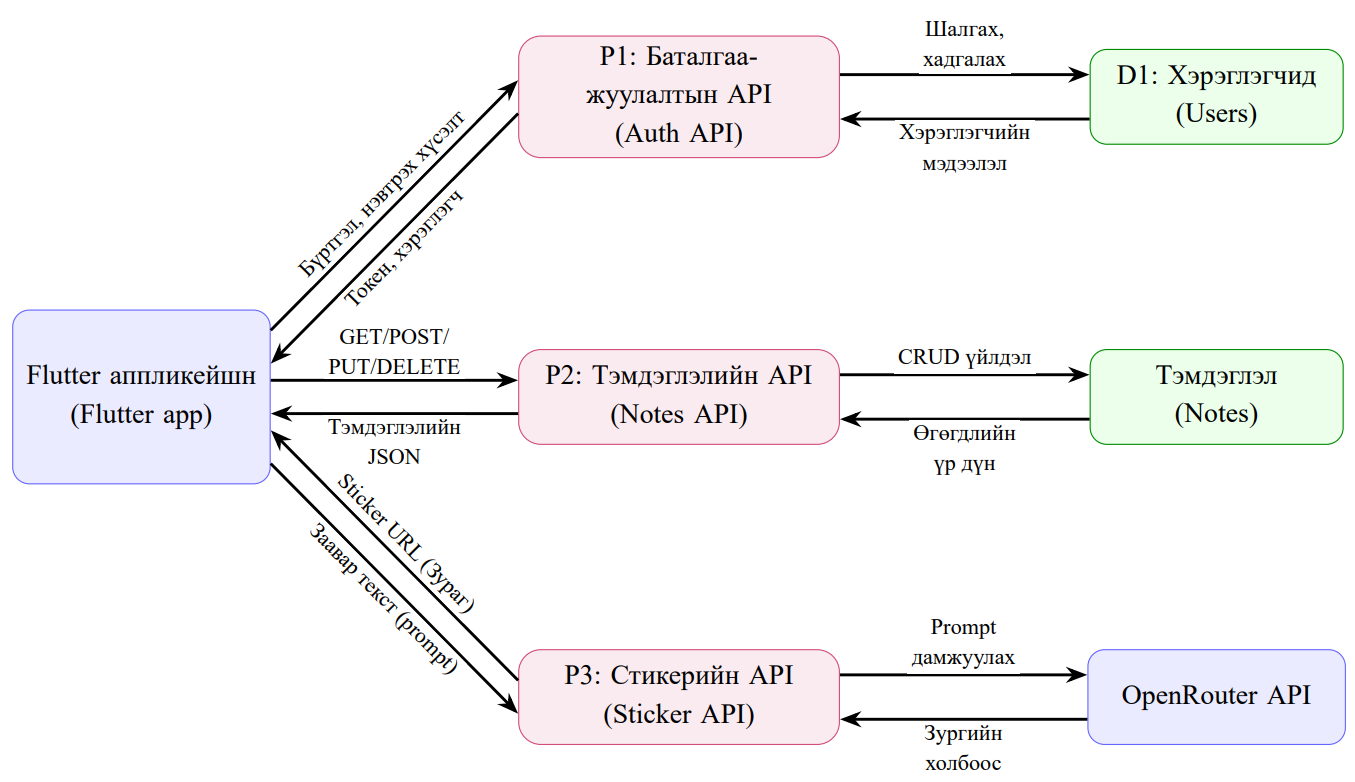
\includegraphics[width=\columnwidth]{Pictures/13.png}
\begin{flushright}
\textit{\small Зураг 2.2 Нэгдүгээр түвшний өгөгдлийн урсгал: сервер талын
модулийн задаргаа}
\end{flushright}

\textbf{3. Судалгааны үр дүн}

Системийн интеграцийн түвшинд гол
урсгалууд амжилттай баталгаажсан.

\vspace{0.2cm}
\begin{flushright}
\textit{\small Хүснэгт 3.1 Интеграцийн туршилтын үр дүнгийн нэгтгэл}
\end{flushright}
\vspace{-0.2cm}
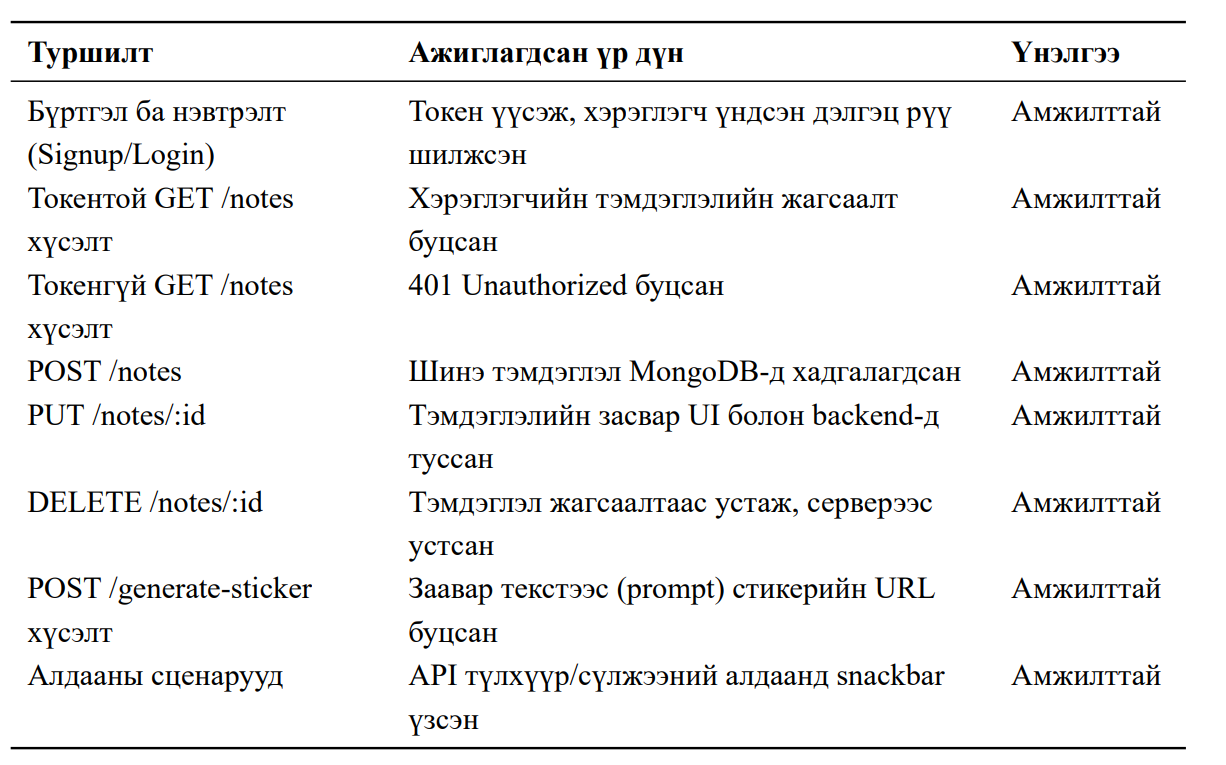
\includegraphics[width=\columnwidth]{Pictures/14.png}

Стикер үүсгэх урсгалд дараах үе шат
баталгаажсан:

\begin{itemize}
\item Клиент талаас POST
/api/notes/generate‐sticker хүсэлтээр prompt
илгээнэ;
\item Backend OpenRouter API руу хүсэлт
дамжуулж зураг үүсгэнэ (model: flux-pro
эсвэл fallback);
\item URL эсвэл алдааны хариу буцаана;
\item Frontend сүүлийн тэмдэглэлийн stickerUrl
талбарт хадгалж, preview харуулна.
\end{itemize}

Гүйцэтгэлийн бодит хэмжилт
S1, S2, S3 туршилтын сценаруудыг бодит
backend орчинд ажиллуулж,
/api/notes/generate‐sticker төгсгөлийн цэгийн
latency болон CPU ачааллыг хэмжив.

\vspace{0.2cm}
\begin{flushright}
\textit{\small Хүснэгт 3.2 Generative AI туршилтын бодит хэмжилтийн үр дүн}
\end{flushright}
\vspace{-0.2cm}
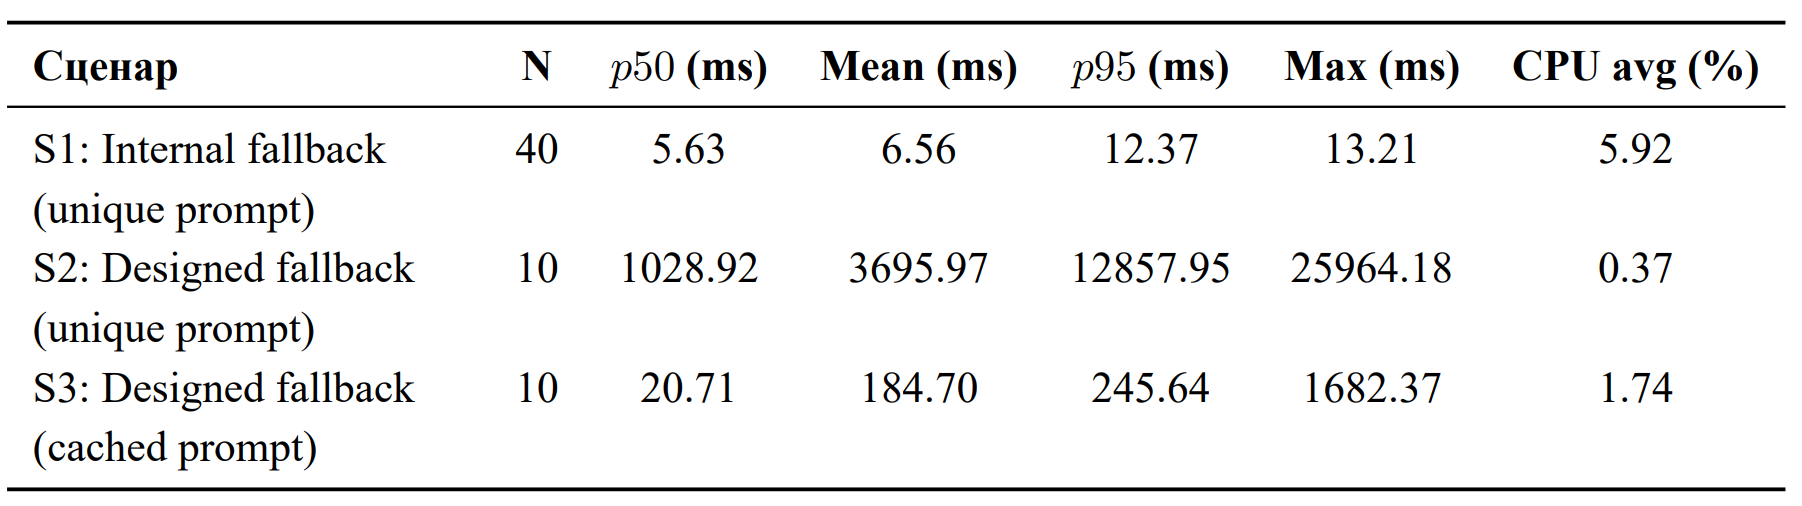
\includegraphics[width=\columnwidth]{Pictures/21.png}

\textbf{4. Дүгнэлт}

Энэхүү судалгааны ажлаар гар утасны
хэрэглээний харагдах хэсэг, сервер талын
хэсэг, өгөгдлийн сан болон хиймэл оюуны
үйлчилгээний нэгтгэлийг ашиглан ``AI
Notebook'' системийг бодит түвшинд
хэрэгжүүлж, тэмдэглэл үүсгэх, унших,
шинэчлэх, устгах үйлдэл болон хиймэл оюун
ухаанаар стикер үүсгэх үндсэн боломжуудыг
нэгтгэн амжилттай туршиж нотолсон.
Судалгааны үр дүнгээс үзэхэд
модульчлагдсан бүтэц, токенд суурилсан
хамгаалалт, өгөгдлийн урсгал болон
дарааллын диаграммын уялдаа холбоо нь
системийн ажиллагааг ойлгомжтой, өргөтгөх
болон хэрэглээнд нэвтрүүлэх боломжтой
шийдэл гэж дүгнэж байна.

\textbf{5. Ном зүй}

[1] Google. Flutter documentation.
https://docs.flutter.dev, 2026.

[2] OpenJS Foundation. Node.js documentation.
https://nodejs.org/en/docs, 2026.

[3] MongoDB Inc. MongoDB manual.

https://www.mongodb.com/docs/manual, 2026.

[4] Michael Jones, John Bradley, and Nat Sakimura.
RFC 7519: JSON Web Token (JWT).
https://www.rfc-editor.org/rfc/rfc7519, 2015.

\end{multicols}




\clearpage
\pagenumbering{arabic}
\setcounter{page}{1}

\addtotoc{Abstract}
\thispagestyle{plain}


\begin{center}
{\Large\bfseries DEVELOPMENT OF A DIGITAL NOTEBOOK APPLICATION}
\end{center}

\begin{flushright}
\small
DEPARTMENT OF COMPUTER SCIENCE

Student: s21c032b, E. Anu\\
Supervisor: U. Anujin
\end{flushright}

\setlength{\columnsep}{5mm}
\setlength{\parindent}{0pt}

\begin{multicols}{2}

\small

\textbf{1. Introduction}

In modern times, people have an increasing need to regularly record their daily tasks, studies,
and personal plans. However, paper-based notes can be easily lost, are inconvenient to carry,
and make information retrieval difficult. At the same time, many existing note-taking applications
have limited reminder and additional features. Therefore, there is a need for an intelligent digital
note-taking solution that can generate stickers, provide reminders, and include a calendar view.

Based on this requirement, this work developed and implemented the “AI Notebook” system.

\textbf{Goal}

The main goal of this research is to design, develop, and evaluate a mobile application for intelligent
note-taking based on frontend and backend architecture, including user authentication, note management,
and AI-based sticker generation.

\textbf{2. Research Methodology}

This research applied the Design Science Research methodology, which includes iterative phases of
requirement analysis, architecture design, system development, testing, and validation.

At the methodological level:
\begin{itemize}
\item Data Flow Diagrams (DFD) were developed at context, level 1, and level 2 to describe system flows.
\item Sequence diagrams were used to model login, note creation, sticker generation, and notification workflows.
\item Integration testing was performed, including API flow testing, token authentication, error handling,
and performance measurement.
\end{itemize}

Functional and non-functional requirements were defined separately, and a traceability matrix was used
to show how each requirement is implemented and verified across modules.

\vspace{0.2cm}
\begin{flushright}
\textit{\small Table 2.1 Functional Requirements Traceability Matrix}
\end{flushright}
\vspace{-0.2cm}
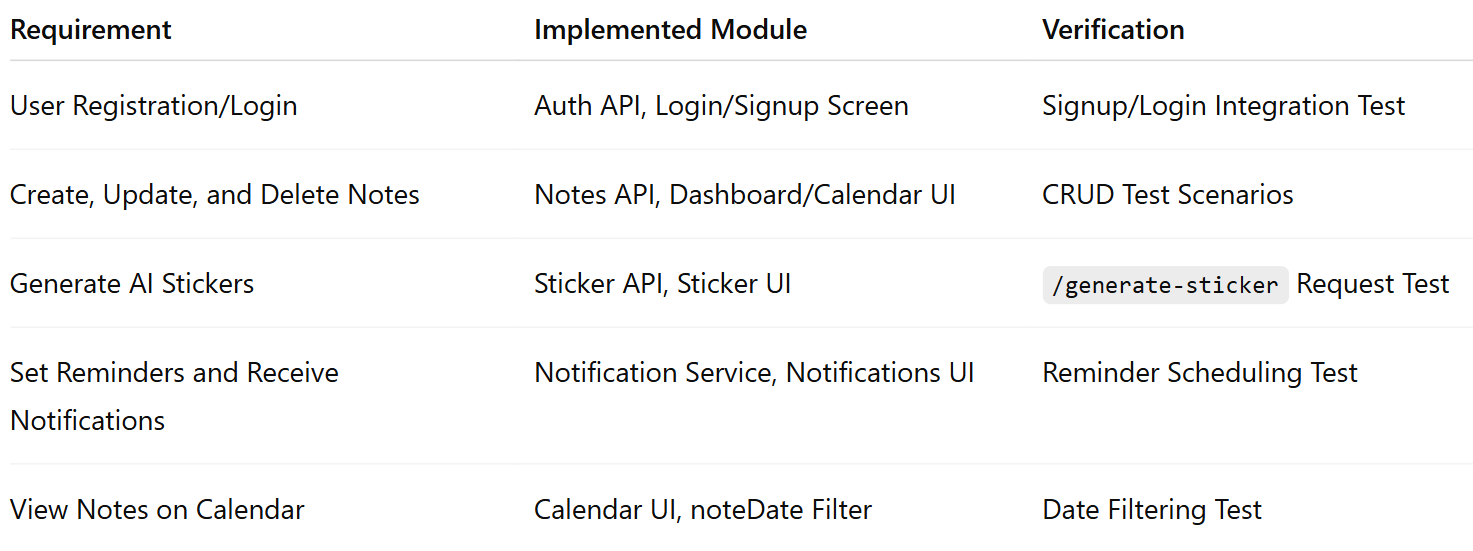
\includegraphics[width=\columnwidth]{Pictures/11.1.png}

In addition, data flows were analyzed from context level down to hierarchical levels (DFD level 0–2),
covering the flow from user actions to database and AI services. The context and level 1 diagrams are
shown below.

\vspace{0.2cm}
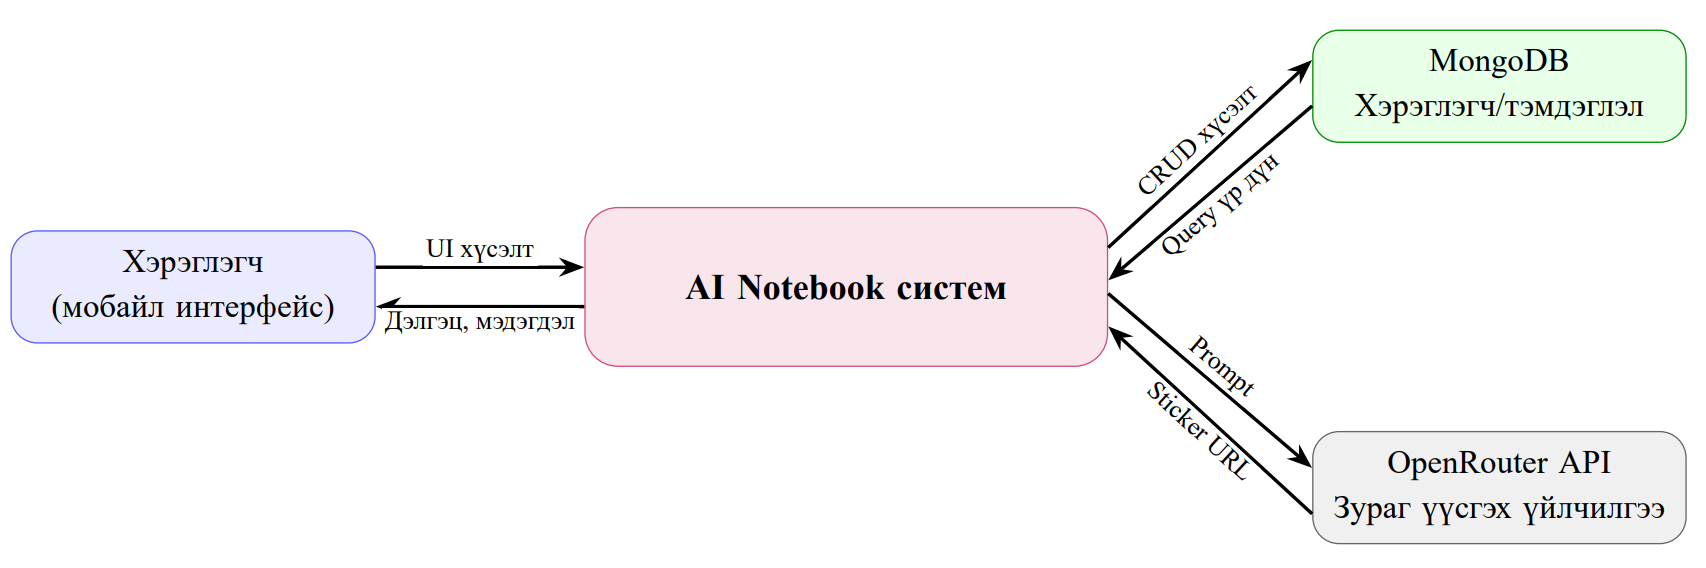
\includegraphics[width=\columnwidth]{Pictures/12.png}
\begin{flushright}
\textit{\small Figure 2.1 Context-Level Data Flow Diagram}
\end{flushright}

\vspace{0.2cm}
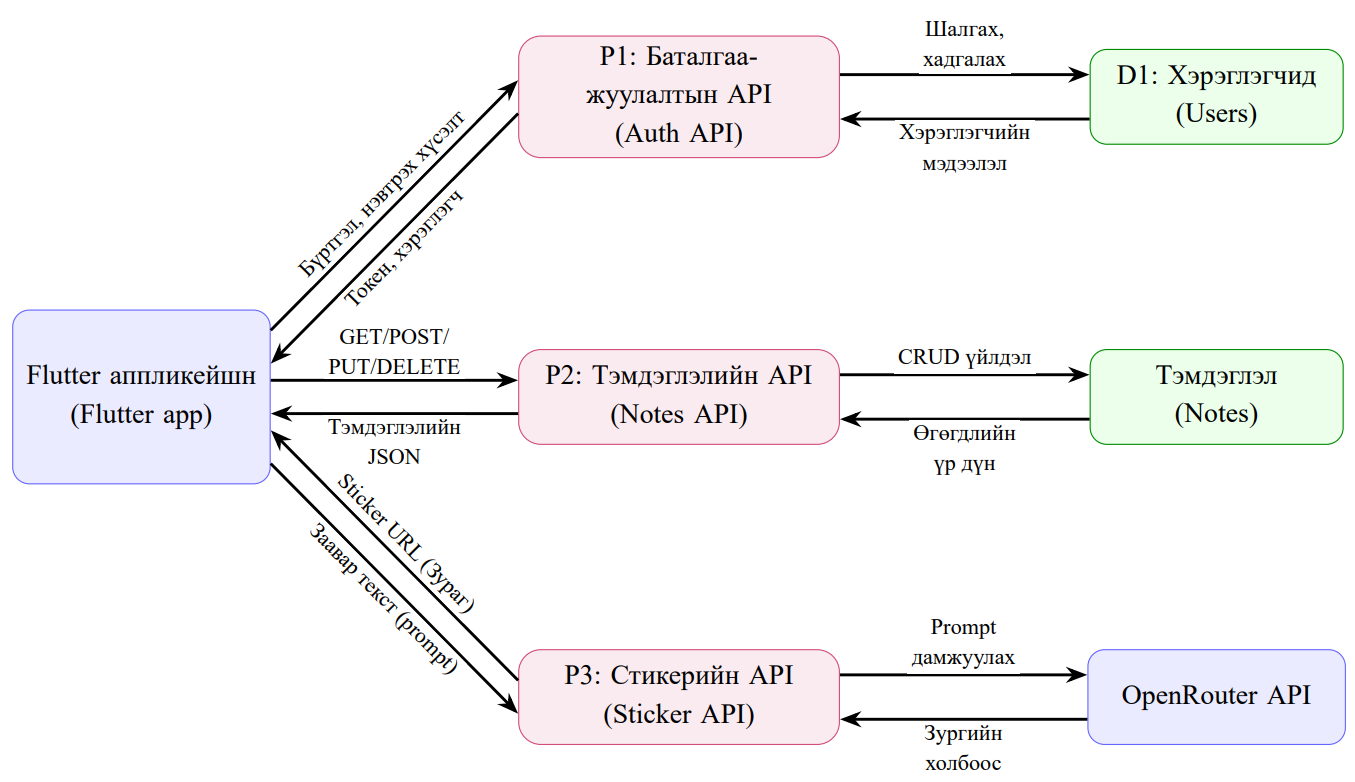
\includegraphics[width=\columnwidth]{Pictures/13.png}
\begin{flushright}
\textit{\small Figure 2.2 Level 1 Data Flow Diagram: Backend Module Decomposition}
\end{flushright}

\textbf{3. Results}

At the system integration level, the main workflows were successfully validated.

\vspace{0.2cm}
\begin{flushright}
\textit{\small Table 3.1 Summary of Integration Testing Results}
\end{flushright}
\vspace{-0.2cm}
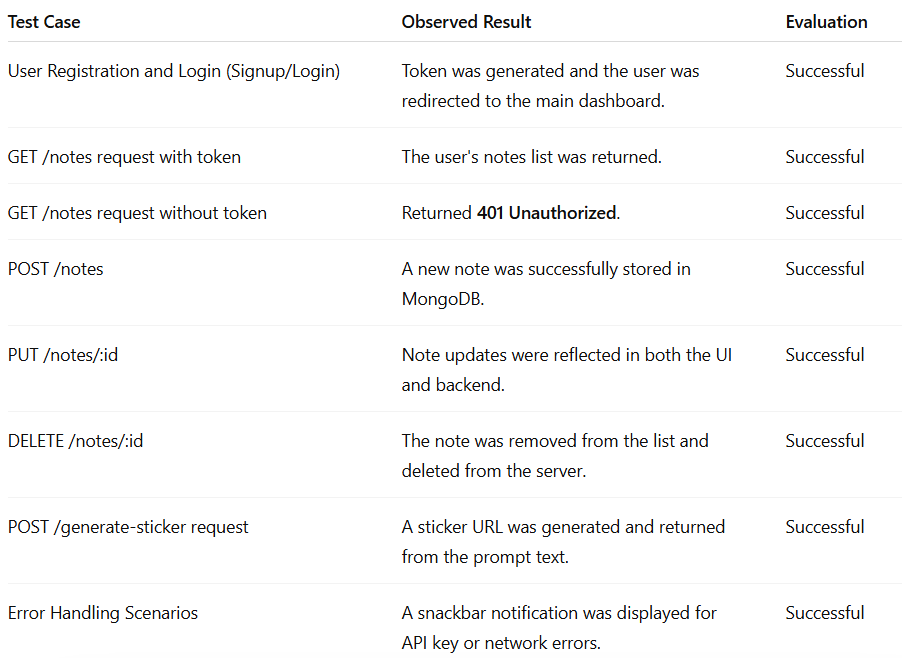
\includegraphics[width=\columnwidth]{Pictures/14.1.png}

The following steps were confirmed in the sticker generation workflow:

\begin{itemize}
\item The client sends a POST request to /api/notes/generate-sticker with a prompt;
\item The backend forwards the request to the OpenRouter API to generate an image (model: flux-pro or fallback);
\item A URL or error response is returned;
\item The frontend stores the stickerUrl in the latest note and displays a preview.
\end{itemize}

Performance measurements were conducted using real backend environments with S1, S2, and S3 test scenarios,
measuring latency and CPU load of the /api/notes/generate-sticker endpoint.

\vspace{0.2cm}
\begin{flushright}
\textit{\small Table 3.2 Real Performance Results of Generative AI Testing}
\end{flushright}
\vspace{-0.2cm}
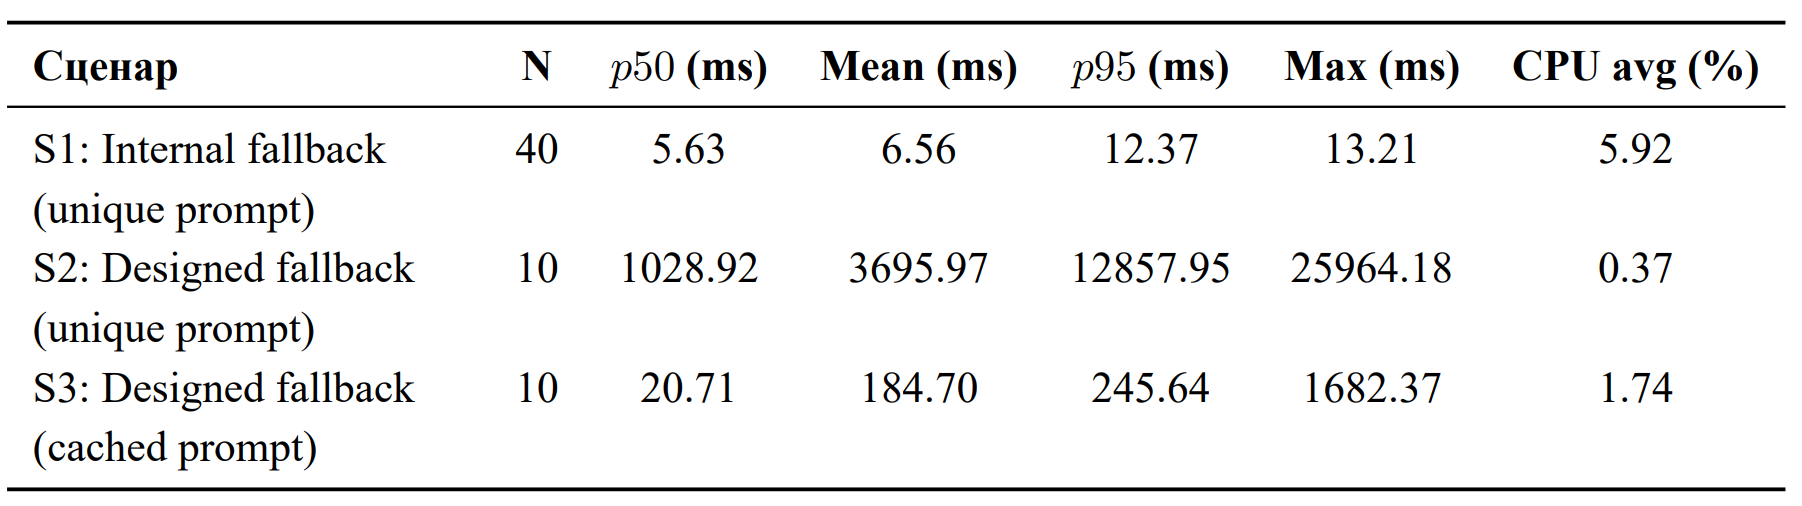
\includegraphics[width=\columnwidth]{Pictures/21.png}

\textbf{4. Conclusion}

This research successfully implemented an “AI Notebook” system by integrating mobile frontend,
backend services, database, and artificial intelligence components. The system supports core features
such as creating, reading, updating, and deleting notes, as well as AI-based sticker generation.

The results show that a modular architecture, token-based authentication, data flow design,
and sequence modeling contribute to a system that is understandable, scalable, and suitable for real-world deployment.

\textbf{5. References}

[1] Google. Flutter documentation.
https://docs.flutter.dev, 2026.

[2] OpenJS Foundation. Node.js documentation.
https://nodejs.org/en/docs, 2026.

[3] MongoDB Inc. MongoDB manual.

https://www.mongodb.com/docs/manual, 2026.

[4] Michael Jones, John Bradley, and Nat Sakimura.
RFC 7519: JSON Web Token (JWT).
https://www.rfc-editor.org/rfc/rfc7519, 2015.

\end{multicols}